\documentclass[journal]{IEEEtran}
\usepackage{graphicx}
\usepackage{url}
\usepackage{amsmath,amssymb}
\usepackage{cite}
\hyphenation{Byte-Net}

\begin{document}

\title{Position Invariant Statistics and Gated Fusion for Robust Multimedia File Fragment Classification}

\author{Payaldurga, Mehul, and Arpita
\thanks{Manuscript prepared for the semester project under the guidance of Prof. Jignesh Patel, Indian Institute of Information Technology Vadodara, India.}
\thanks{The authors are with the Indian Institute of Information Technology Vadodara, Gujarat, India (e-mail: 202351103@iiitvadodara.ac.in).}}

\markboth{IEEE Signal Processing Letters}
{Payaldurga \MakeLowercase{\textit{et al.}}: Position Invariant Statistics and Gated Fusion for File Fragment Classification}

\maketitle

\begin{abstract}
Multimedia file fragment classification identifies the type of a file from a short block of raw bytes without any metadata. A recent method, ByteNet, converts each fragment into a grayscale image through bit shifting and combines an image branch with a byte branch that reads the raw bytes by position. We reproduce this method on a seven class dataset built from real files and find that the byte branch carries almost no information when fragments start at arbitrary offsets, reaching only twenty two percent accuracy alone. We replace it with a position invariant branch that summarizes the byte histogram and the entropy of the fragment, and we merge the two branches with a learned sigmoid gate. Over three random seeds, the extension improves accuracy from 71.9 to 77.2 percent, lifts a transformer variant from 53.2 to 78.1 percent, and loses only five points when thirty percent of the bytes are corrupted, where the original model loses twenty.
\end{abstract}

\begin{IEEEkeywords}
Convolutional neural networks, file fragment classification, gated fusion, multimedia forensics, robustness.
\end{IEEEkeywords}

\IEEEpeerreviewmaketitle

\section{Introduction}
\IEEEPARstart{W}{hen} a storage device is damaged, formatted, or carved for evidence, file system metadata is often gone and only unlabeled blocks of bytes remain. Deciding what type of file each block came from is the task of multimedia file fragment classification. Classical approaches use byte frequency, entropy, and other statistics with a shallow classifier, and neural approaches treat the fragment as a one dimensional sequence \cite{bytenet}.

Liu \textit{et al.} proposed ByteNet, which looks inside the bytes rather than only between them \cite{bytenet}. Their Byte2Image model shifts the bits of each byte, stacks the shifted copies, and applies an intrabyte n-gram window, so that a fragment of $N_s$ bytes becomes a grayscale image. A deep image branch learns from this picture, and a shallow byte branch learns from the raw bytes. Their features are concatenated before a softmax layer.

We reproduced this pipeline and studied which part of it does the work. Our contribution is a small change with a measurable effect. First, we show that the shallow byte branch is nearly uninformative when a fragment can begin anywhere inside a file, because it assigns a separate weight to every byte position. Second, we replace it with a statistics branch built from the byte histogram and entropy, which does not depend on position. Third, we fuse the two branches with a learned gate and evaluate robustness to random byte corruption, a situation common in damaged media that the original work does not test.

\section{Related Work}
Early fragment classifiers computed byte frequency, entropy, and compression based features and fed them to support vector machines. Conti \textit{et al.} classified fragments of large binary objects with such primitive features \cite{conti}, and Fitzgerald \textit{et al.} borrowed language processing ideas, using byte n-grams as vocabulary \cite{fitz}. These methods ignore position by construction, since a frequency count does not record where a byte occurred.

Neural methods later replaced hand designed features. Convolutional and residual networks read the byte sequence directly \cite{resnet}, and transformer style networks built from simple token mixing blocks have been tried as well \cite{poolformer}. ByteNet sits in this line, adding the visual view of the intrabyte bits and a shallow side branch \cite{bytenet}. Our work revisits a design question that earlier statistical methods answered differently: whether position information should be given to the classifier at all when the starting offset of a fragment is unknown.

\section{Existing Work and Problem Statement}
\subsection{Byte2Image and ByteNet}
Let a fragment be $\mathbf{x}=(x_1,\dots,x_{N_s})$ with $x_j\in\{0,\dots,255\}$. Byte2Image forms $x^{(i)}=(x^{(i-1)}\ll 1)\bmod 256$ for $i=1,\dots,7$, which exposes every bit to the most significant position in turn, and stacks the eight versions into an $N_s\times 8$ matrix. An intrabyte n-gram then slides a window of $n$ rows and flattens it, giving an image of size $(N_s-n+1)\times 8n$. Fig.~\ref{fig:b2i} shows examples from four file types. Structure such as the regular columns of source code and the dense texture of compressed image data is visible by eye.

ByteNet has two branches. The image branch has four stages of residual blocks (ByteResNet) or pooling based transformer blocks (ByteFormer). The byte branch is a fully connected layer applied to the raw byte vector. The two feature vectors are concatenated and sent to a softmax layer. Training uses AdamW with weight decay 0.01, a cosine schedule with warmup, mixup, flipping, and random erasing \cite{adamw,mixup}.

\subsection{Problem}
The byte branch multiplies the byte at position $j$ by its own weight. This helps when every fragment starts at a fixed place, for example at the start of a file where headers appear. Practical fragments are cut at arbitrary offsets, so a given file type does not place a given value at a given position. The branch then has a large number of weights and no stable signal to learn from. The problem we address is to supply the second branch with information that survives an unknown starting offset and remains useful when some bytes are damaged.

\begin{figure}[t]
\centering
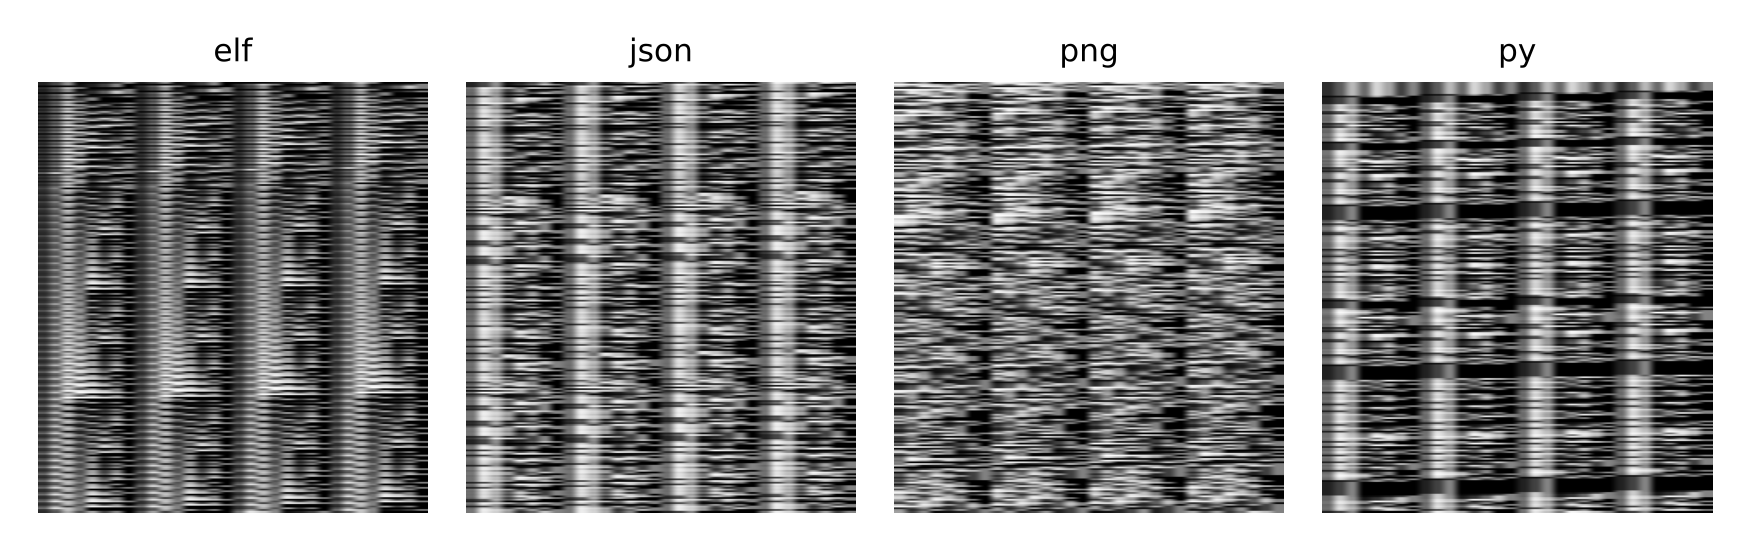
\includegraphics[width=\columnwidth]{figs/fig_b2i.png}
\caption{Byte2Image outputs for one fragment each of four file types, with $n=4$.}
\label{fig:b2i}
\end{figure}

\section{Proposed Extension}
\subsection{Position invariant statistics branch}
For a fragment $\mathbf{x}$ we compute the normalized histogram $h_k=\frac{1}{N_s}\sum_j \mathbb{1}[x_j=k]$ for $k=0,\dots,255$ and the Shannon entropy $H=-\sum_k h_k\log_2 h_k$. The statistics vector is
\begin{equation}
\mathbf{s}=\big[\,16\,h_0,\dots,16\,h_{255},\;H/8\,\big]\in\mathbb{R}^{257},
\end{equation}
where the factor 16 brings typical histogram values to a scale near one. Reordering the bytes does not change $\mathbf{s}$, so the starting offset has no effect on it. A two layer perceptron maps $\mathbf{s}$ to a 128 dimensional feature $\mathbf{f}_s$. This replaces the position dependent byte branch.

\subsection{Gated fusion}
Let $\mathbf{f}_i$ be the image branch feature. Both features are projected to $d=128$ dimensions, giving $\mathbf{p}_s$ and $\mathbf{p}_i$. A gate computed from both decides how much of each to pass on:
\begin{equation}
\mathbf{g}=\sigma\!\big(\mathbf{W}[\mathbf{p}_s;\mathbf{p}_i]+\mathbf{b}\big),\qquad
\mathbf{z}=\big[\,\mathbf{g}_{1:d}\odot\mathbf{p}_s;\;\mathbf{g}_{d+1:2d}\odot\mathbf{p}_i\,\big],
\end{equation}
and $\mathbf{z}$ goes to the softmax layer. The idea follows gated multimodal units \cite{gmu}. When a fragment is damaged, the gate can lower the weight of the branch that has become unreliable, which plain concatenation cannot do. Fig.~\ref{fig:arch} shows the full model.

\begin{figure}[t]
\centering
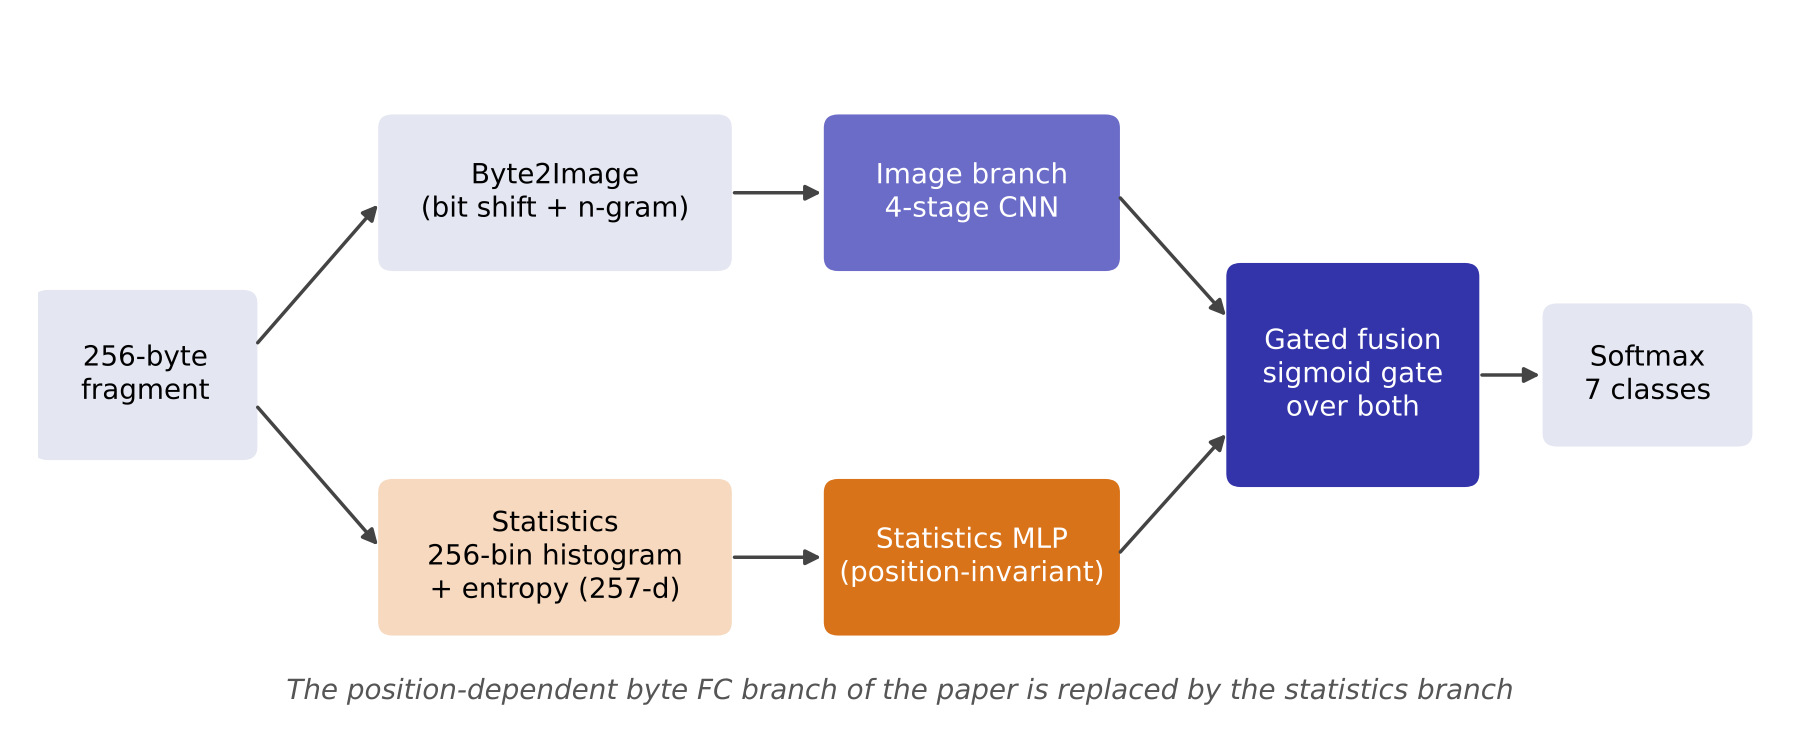
\includegraphics[width=\columnwidth]{figs/fig_arch.png}
\caption{Proposed model. The statistics branch replaces the byte branch and the two feature vectors are merged by a learned gate.}
\label{fig:arch}
\end{figure}

\subsection{Robustness protocol}
After training, we flip a fraction $r\in\{0,0.05,0.10,0.20,0.30\}$ of the bytes of every test fragment to random values and measure accuracy. The models are not retrained or trained with corruption, so the test measures how the learned features degrade.

\section{Experiments}
\subsection{Hyperparameters}
Table~\ref{tab:hp} lists the settings shared by all runs. The extension adds only the statistics multilayer perceptron and the gate, so the image branch and the optimization recipe are identical to the baseline. This keeps the comparison to a single change in the second branch.

\begin{table}[t]
\caption{Training Settings Shared by All Configurations}
\label{tab:hp}
\centering
\begin{tabular}{ll}
\hline
Setting & Value \\
\hline
Optimizer & AdamW, weight decay 0.01 \\
Learning rate & $5\times10^{-4}$, cosine decay with warmup \\
Loss & Negative log likelihood on mixup labels \\
Batch size & 64 \\
Stage channels & $[16, 32, 64, 128]$ \\
Epochs & 16 (ByteResNet), 60 (ByteFormer) \\
Fragment length & 256 bytes \\
n-gram size & 4 \\
Fusion width $d$ & 128 \\
\hline
\end{tabular}
\end{table}

\subsection{Setup}
No public copy of the original benchmark was available to us offline, so we built a dataset from real files on the machine: ELF binaries, gzip archives, HTML, JSON, PDF, PNG, and Python source. Each file contributes up to 320 fragments of 256 bytes taken at random offsets, for 2,240 fragments in total, split 80/20 into 1,792 training and 448 test fragments with a fixed seed. Models use channels $[16,32,64,128]$, depth one, batch size 64, learning rate $5\times10^{-4}$, and 16 epochs (60 for ByteFormer), on a single CPU core. Every configuration is trained with three seeds and we report the mean and standard deviation. With 448 test fragments, one standard error of a single accuracy is about two points, so differences below this level should not be read as real.

Fragments are sampled by choosing a source file at random, a random offset inside it, and reading 256 bytes. Byte2Image images and statistics vectors are computed once before training. Training uses horizontal flipping and random erasing on the images, and mixup with a Beta parameter of 0.8 on all inputs together with the labels. The corruption test uses the same fragments and the same trained weights for every rate, with a fixed seed for the random byte positions.

Absolute numbers are not comparable with those in the original paper, which uses a larger benchmark and a different class set. Our comparison is between models trained on the same data. The baseline reaches 71.9 percent here, while an earlier run on a previous build of the dataset gave 73.4 percent, which shows that the data build alone moves accuracy by more than one point.

\begin{table}[t]
\caption{Composition of the Fragment Dataset}
\label{tab:data}
\centering
\begin{tabular}{lcc}
\hline
Class & Source files scanned & Fragments used \\
\hline
ELF binary & 4,000 & 320 \\
gzip archive & 1,543 & 320 \\
HTML & 448 & 320 \\
JSON & 3,173 & 320 \\
PDF & 525 & 320 \\
PNG & 561 & 320 \\
Python source & 4,000 & 320 \\
\hline
\end{tabular}
\end{table}

\begin{table}[t]
\caption{Test Accuracy Over Three Seeds (Percent)}
\label{tab:main}
\centering
\begin{tabular}{lrc}
\hline
Configuration & Params & Accuracy \\
\hline
ByteResNet baseline (byte + image) & 488,695 & $71.9\pm1.2$ \\
Image branch only & 488,695 & $73.3\pm1.9$ \\
Byte branch only & 488,695 & $22.2\pm0.9$ \\
Statistics branch only & 505,335 & $74.9\pm2.8$ \\
Statistics + image, concatenation & 505,335 & $\mathbf{77.2\pm1.7}$ \\
Statistics + image, gated & 604,151 & $77.1\pm3.8$ \\
\hline
ByteFormer baseline & 185,911 & $53.2\pm1.9$ \\
ByteFormer + statistics, gated & 301,367 & $\mathbf{78.1\pm1.2}$ \\
\hline
\end{tabular}
\end{table}

\subsection{Accuracy}
Table~\ref{tab:main} gives the results. The byte branch alone reaches 22.2 percent, above the 14 percent expected from guessing among seven classes but far below any other branch, which confirms the problem stated above. The statistics branch alone reaches 74.9 percent, which is at least as good as the image branch alone at 73.3 percent. Adding statistics to the image branch gives 77.2 percent, and the gain over the baseline is positive in each seed, at 4.9, 5.1, and 5.8 points, a mean of 5.3 points.

\begin{table}[t]
\caption{Per Class Test Accuracy (Percent, Pooled Over Three Seeds)}
\label{tab:class}
\centering
\begin{tabular}{lccccccc}
\hline
 & ELF & gz & HTML & JSON & PDF & PNG & Py \\
\hline
Baseline & 78 & \textbf{95} & 79 & 84 & 55 & 24 & 86 \\
Stat. + image & \textbf{81} & 79 & \textbf{86} & \textbf{89} & \textbf{56} & \textbf{52} & \textbf{95} \\
Stat. + image + gate & \textbf{82} & 83 & \textbf{85} & \textbf{89} & \textbf{56} & 47 & \textbf{95} \\
\hline
\end{tabular}
\end{table}

\begin{figure}[t]
\centering
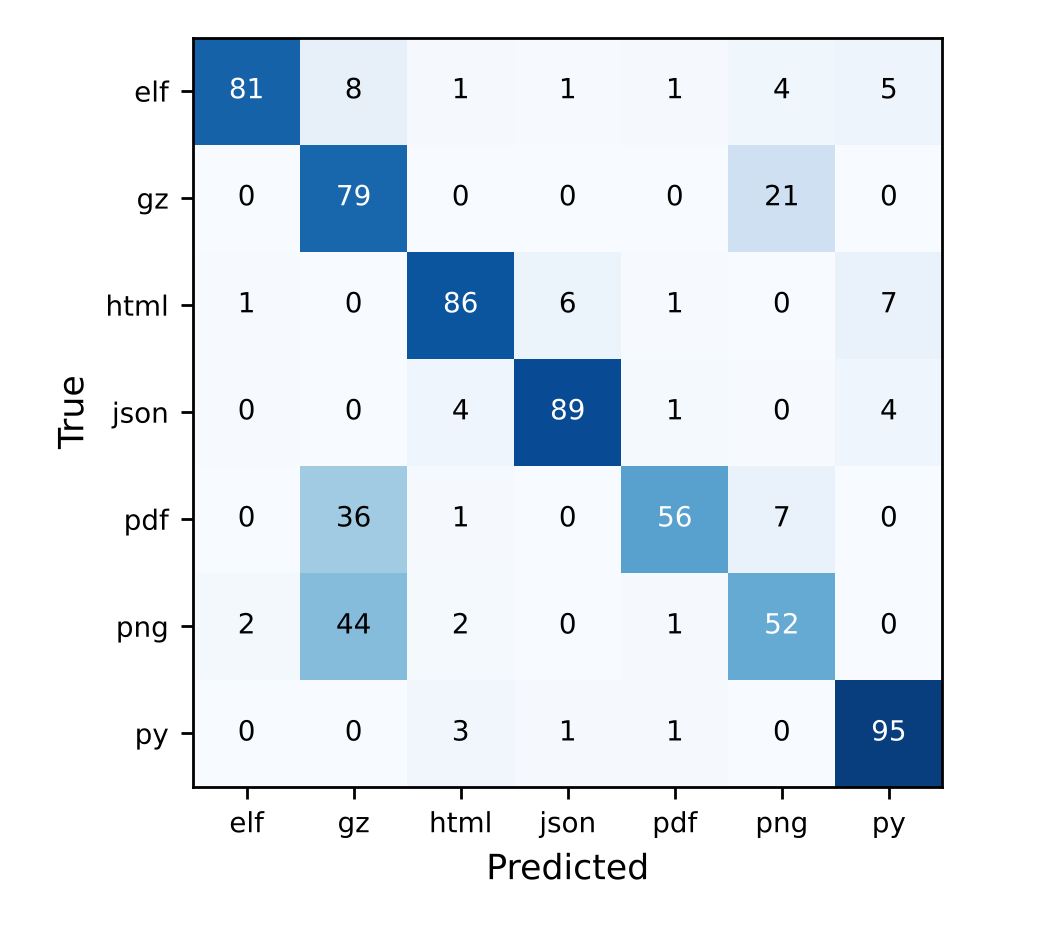
\includegraphics[width=0.85\columnwidth]{figs/fig_cm.png}
\caption{Row normalized confusion matrix (percent) of the statistics plus image model, pooled over three seeds.}
\label{fig:cm}
\end{figure}

Table~\ref{tab:class} and Fig.~\ref{fig:cm} show where the gain comes from. The largest improvement is on PNG, from 24 to 52 percent, followed by Python source, from 86 to 95 percent. The change is not uniform: gzip falls from 95 to 79 percent. PNG, gzip, and many PDF streams are all compressed, so their histograms are nearly flat and hard to tell apart. Of the PNG fragments, 44 percent are labeled as gzip, and 36 percent of PDF fragments are labeled as gzip. The image branch of the baseline, trained together with the position branch, separated gzip better, probably because of the regular block framing of deflate data that a histogram does not capture. The gain therefore comes from classes with distinct byte distributions and is partly paid for on compressed classes.

\begin{table}[t]
\caption{Paired Accuracy Gain Over the Baseline (Percentage Points)}
\label{tab:paired}
\centering
\begin{tabular}{lcccc}
\hline
Configuration & Seed 1 & Seed 2 & Seed 3 & Mean \\
\hline
Statistics only & $+1.1$ & $+4.0$ & $+4.0$ & $+3.1$ \\
Statistics + image & $+4.9$ & $+5.1$ & $+5.8$ & $+5.3$ \\
Statistics + image + gate & $+2.5$ & $+5.6$ & $+7.6$ & $+5.2$ \\
\hline
\end{tabular}
\end{table}

Each seed fixes the train and test split and the initial weights, so Table~\ref{tab:paired} compares models on identical data. The statistics plus image model gains in every seed with a narrow range, while the gated model has a wider range from 2.5 to 7.6 points, which explains its larger standard deviation in Table~\ref{tab:main}.

The gate did not improve on plain concatenation. Its mean is 77.1 percent with a larger spread, and its paired gains over the baseline were 2.5, 5.6, and 7.6 points. We therefore do not claim that the gate raises clean accuracy. The transformer variant gains the most, rising from 53.2 to 78.1 percent. With few training fragments and only 16 to 60 epochs, the pooling based network learns slowly from the image alone, and the statistics branch supplies a strong signal that does not need to be learned from pixels.

\subsection{Robustness}
\begin{table}[t]
\caption{Test Accuracy Under Byte Corruption (Percent, Mean of Three Seeds)}
\label{tab:rob}
\centering
\begin{tabular}{lccccc}
\hline
Corrupted bytes & 0\% & 5\% & 10\% & 20\% & 30\% \\
\hline
Baseline & 71.9 & 71.0 & 68.3 & 61.5 & 52.3 \\
Image only & 73.3 & 71.5 & 70.2 & 62.4 & 52.9 \\
Statistics only & 74.9 & 74.9 & 74.4 & 73.4 & 73.0 \\
Statistics + image & 77.2 & 76.4 & 75.9 & 73.6 & 72.4 \\
Statistics + image + gate & 77.1 & 77.3 & 76.3 & 74.7 & 72.4 \\
\hline
ByteFormer baseline & 53.2 & 52.4 & 51.9 & 49.7 & 46.4 \\
ByteFormer + stat. + gate & 78.1 & 77.7 & 76.6 & 75.3 & 73.1 \\
\hline
\end{tabular}
\end{table}

\begin{figure}[t]
\centering
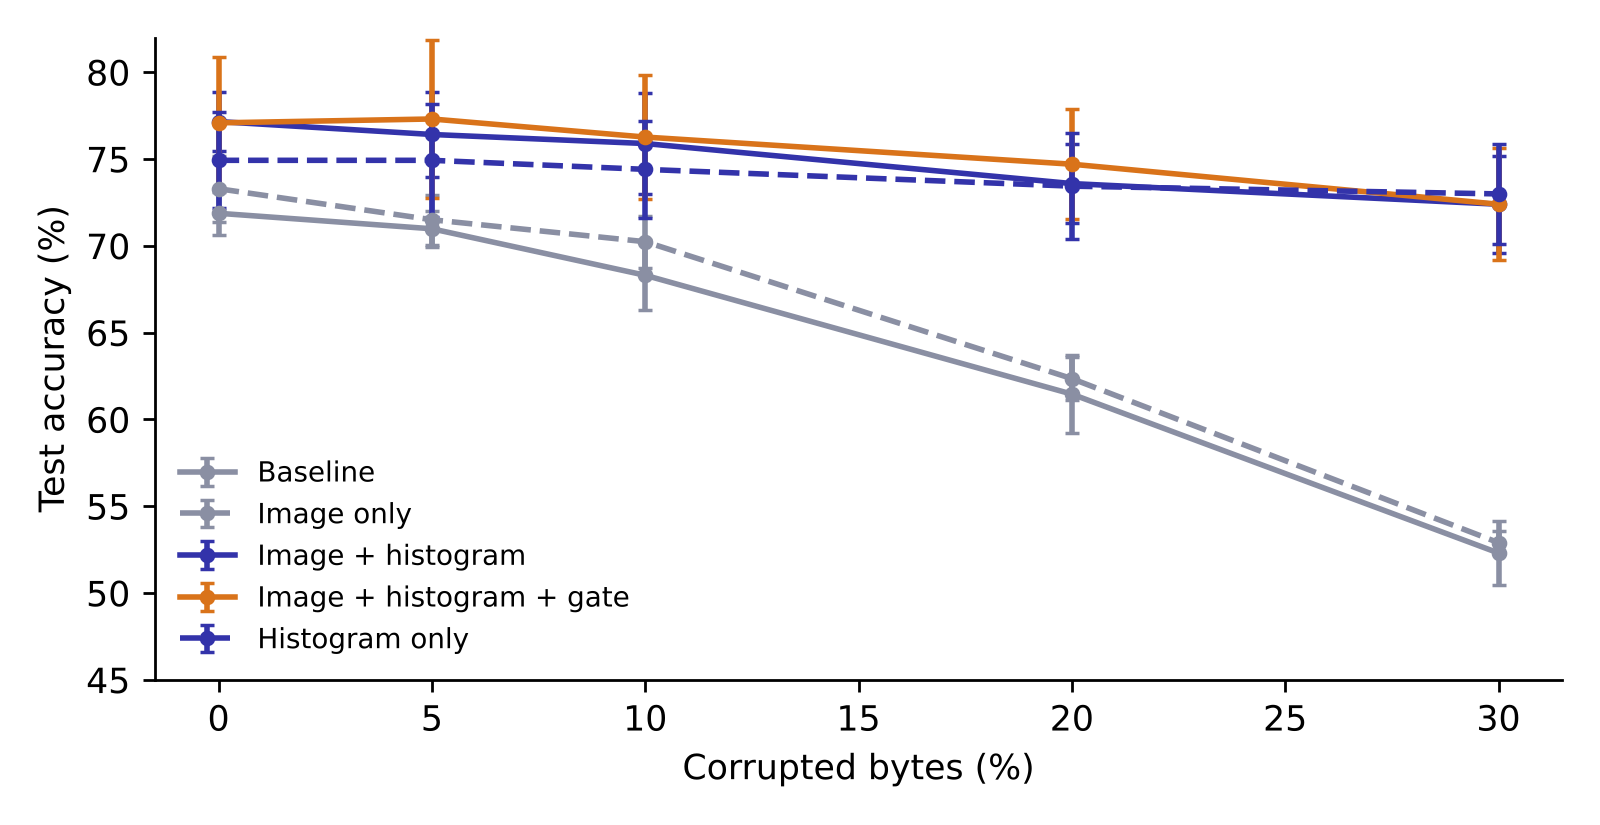
\includegraphics[width=\columnwidth]{figs/fig_rob.png}
\caption{Accuracy against the share of corrupted bytes. Bars show one standard deviation over three seeds.}
\label{fig:rob}
\end{figure}

Table~\ref{tab:rob} and Fig.~\ref{fig:rob} show the effect of corruption. The baseline drops from 71.9 to 52.3 percent at 30 percent corruption, a loss of 19.6 points. The extension drops from 77.2 to 72.4 percent, a loss of 4.8 points. The image branch is sensitive because random bytes change the local bit patterns that its filters rely on. A histogram changes smoothly, since each corrupted byte moves only a small amount of mass between bins. The gated model is slightly higher than concatenation at 5, 10, and 20 percent corruption, but the gaps are within one standard deviation, so this is suggestive rather than established.

\begin{figure}[!t]
\centering
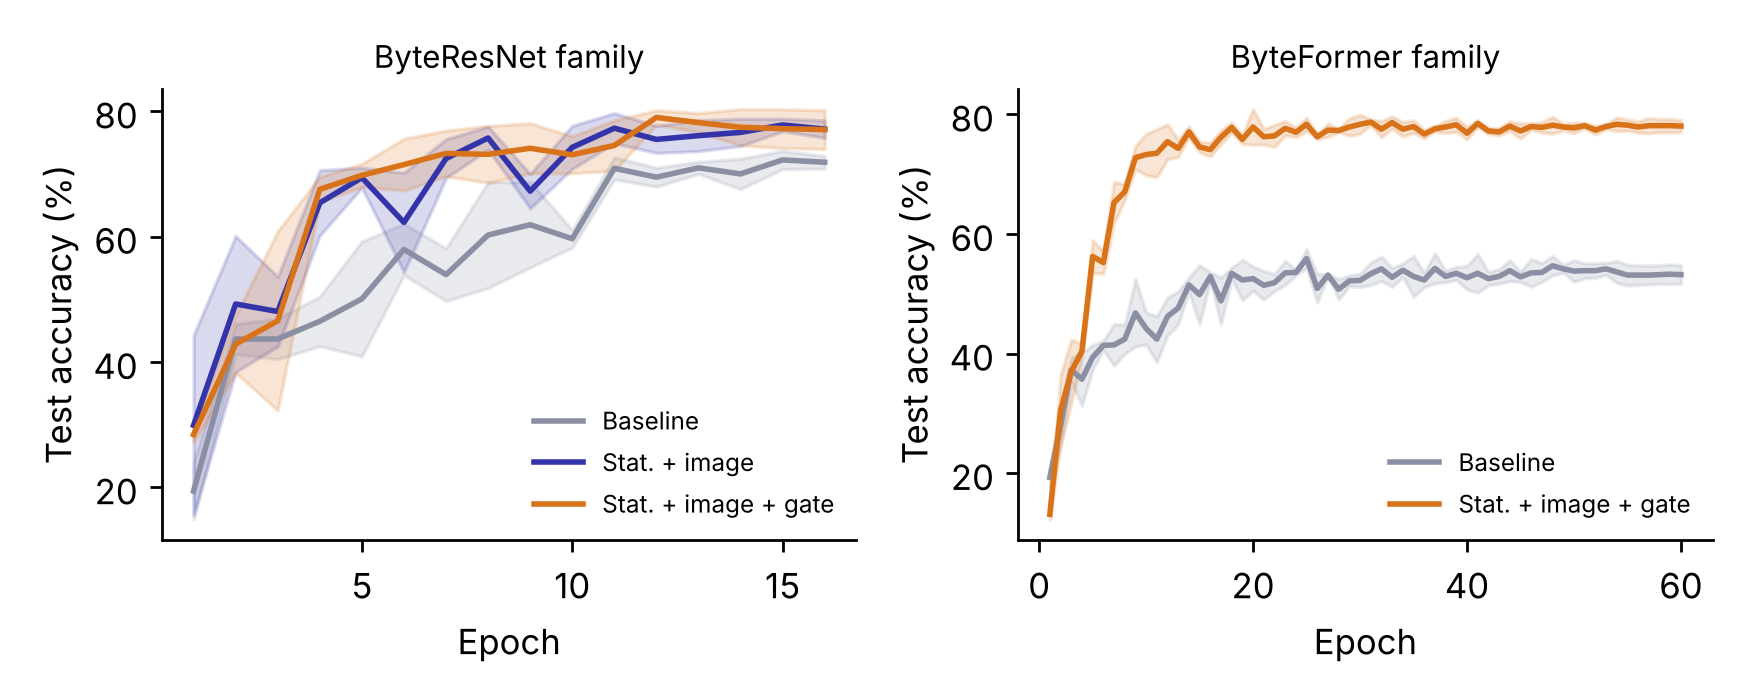
\includegraphics[width=\columnwidth]{figs/fig_curve.png}
\caption{Test accuracy during training, mean and one standard deviation over three seeds.}
\label{fig:curve}
\end{figure}

Fig.~\ref{fig:curve} shows that the statistics branch changes the speed of learning as well as the final value. The ByteFormer baseline needs about 20 epochs to reach 52 percent, while the extended version is at 56 percent after 5 epochs and 73 percent after 10, because the histogram is available from the start. The ByteResNet curves have not fully flattened after 16 epochs, so longer training could reduce the gaps in both directions, and we did not run it.

\subsection{Why the Gate Does Not Help on Clean Data}
We offer a likely explanation and did not test it directly. With 1,792 training fragments, the gate adds 99 thousand parameters, about 20 percent more than the concatenation model, and its output depends on a product of two learned quantities. A small training set gives the gate little to learn from, so it may settle near a constant mixture that behaves like concatenation. The slightly better numbers under corruption are consistent with some learned weighting, but we did not inspect the gate values, and doing so is a clear next step.

\subsection{Reproducibility}
Data preparation, training, and the corruption test are separate Python scripts that take a seed and a configuration name, and each run writes its results to one file from which this letter's numbers are aggregated. A run takes about four minutes on one CPU core.

\subsection{Limits}
The statistics branch alone is within the noise of the full model, so on this dataset most of the useful signal comes from the histogram and the image branch adds at most a small gain. Three seeds cannot separate effects smaller than about two points, and we did not test on the original benchmark.

\subsection{Threats to Validity}
Four points limit how far the results travel. The dataset comes from one machine, so the files share software versions and authorship habits, and a classifier might partly learn those. The split is by fragment, not by file, so two fragments from the same file can fall on both sides of the split, which tends to raise all accuracies and could favor models that memorize file specific statistics. Only one fragment length was tested, and a histogram of 256 bytes over 256 bins is sparse, which may be why the histogram alone does not exceed the combined model. Finally, the corruption we apply is uniform random replacement, while real damage is often a burst of consecutive bytes, which would affect the image and the histogram differently.

\section{Discussion}
The main practical lesson is about where side information belongs in a fragment classifier. A branch that assigns one weight per byte position is appropriate for the first sector of a file, where headers sit at known places, and inappropriate for a sector from the middle of a file. A forensic tool rarely knows which case it faces, so a classifier that uses only position free evidence for the second branch is the safer default, and a position aware branch can be added later when the fragment is known to be a file start.

The robustness result also has a simple reading. The image branch works from local bit patterns, and uniform noise destroys exactly these patterns. The histogram averages over the whole fragment, so noise acts on it as a smooth blend toward a flat distribution. A model that relies on both is protected when the image view fails. This suggests training the image branch with corrupted inputs as the next step, since the image branch then has a chance to learn features that tolerate noise, while the statistics branch already does.

The result for the transformer variant should be read with care. Its baseline is weak in our setting, 53.2 percent, because it has fewer parameters and sees few images, so the large gain partly measures how much that baseline was starved of signal. On the original benchmark, which has many more training fragments, we expect the gap to shrink.

\section{Conclusion}
The byte branch of ByteNet is almost useless when fragments start at random offsets. Replacing it with a histogram and entropy branch raised accuracy by about five points on our data, raised a transformer variant by twenty five points, and cut the loss under thirty percent byte corruption from twenty points to five. Gated fusion was not better than concatenation on clean data. Future work should repeat the study on the original benchmark, with longer fragments, and train with corruption to see whether the image branch can recover its robustness.

\section*{Acknowledgment}
The authors thank Prof. Jignesh Patel for guidance throughout the project.

\begin{thebibliography}{1}
\bibitem{bytenet}
W. Liu, K. Wu, T. Liu, Y. Wang, K.-H. Yap, and L.-P. Chau, ``ByteNet: Rethinking multimedia file fragment classification through visual perspectives,'' \emph{IEEE Trans. Multimedia}, vol. 27, pp. 1305--1318, 2025.

\bibitem{conti}
G. Conti \textit{et al.}, ``Automated mapping of large binary objects using primitive fragment type classification,'' \emph{Digit. Investigation}, vol. 7, pp. S3--S12, 2010.

\bibitem{fitz}
S. Fitzgerald, G. Mathews, C. Morris, and O. Zhulyn, ``Using NLP techniques for file fragment classification,'' \emph{Digit. Investigation}, vol. 9, pp. S44--S49, 2012.

\bibitem{resnet}
K. He, X. Zhang, S. Ren, and J. Sun, ``Deep residual learning for image recognition,'' in \emph{Proc. IEEE Conf. Comput. Vis. Pattern Recognit.}, 2016, pp. 770--778.

\bibitem{poolformer}
W. Yu \textit{et al.}, ``MetaFormer is actually what you need for vision,'' in \emph{Proc. IEEE/CVF Conf. Comput. Vis. Pattern Recognit.}, 2022, pp. 10819--10829.

\bibitem{adamw}
I. Loshchilov and F. Hutter, ``Decoupled weight decay regularization,'' in \emph{Proc. Int. Conf. Learn. Representations}, 2019.

\bibitem{mixup}
H. Zhang, M. Cisse, Y. N. Dauphin, and D. Lopez-Paz, ``mixup: Beyond empirical risk minimization,'' in \emph{Proc. Int. Conf. Learn. Representations}, 2018.

\bibitem{gmu}
J. Arevalo, T. Solorio, M. Montes-y-G\'omez, and F. A. Gonz\'alez, ``Gated multimodal units for information fusion,'' in \emph{Proc. Int. Conf. Learn. Representations Workshop}, 2017.
\end{thebibliography}

\end{document}
